\documentclass[11pt]{article}
\usepackage[margin=1in]{geometry}
\usepackage{amsmath,amssymb,amsthm}
\usepackage{graphicx}
\usepackage{hyperref}
\hypersetup{colorlinks=true,linkcolor=blue,citecolor=blue,urlcolor=blue}

\newtheorem{theorem}{Theorem}
\newcommand{\F}{\mathcal F}
\newcommand{\C}{\mathbb C}

\title{Problem 3.31 has the uncertainty inequality facing the wrong way}
\author{A full counterexample to a problem in arXiv:2107.09057}
\date{13 August 2026}

\begin{document}
\maketitle

\noindent\textbf{Status.}
Full counterexample, high confidence.  Problem~3.31 as printed is false even
for the group-subfactor planar algebra of $\mathbb Z_2$.  Its premise is
automatically satisfied by every normalized $2$-box.  The likely intended
near-minimizer condition has the opposite inequality sign.

\section{Source problem}

The source is Wu, \emph{Quantum smooth uncertainty principles for von
Neumann bi-algebras}~\cite{source}.  Problem~3.31 on source PDF page~15 asks
for a positive function $C(\epsilon,\delta)\to0$ as $\epsilon\to0$ such that
\begin{equation}\label{eq:source}
 H(|x|^2)+H(|\F(x)|^2)\ge 2\log\delta-\epsilon
\end{equation}
forces every normalized $2$-box $x$ of every irreducible subfactor planar
algebra of Jones index $\delta^2$ to lie within $C(\epsilon,\delta)$ of a
bi-shift of a biprojection:

\begin{center}
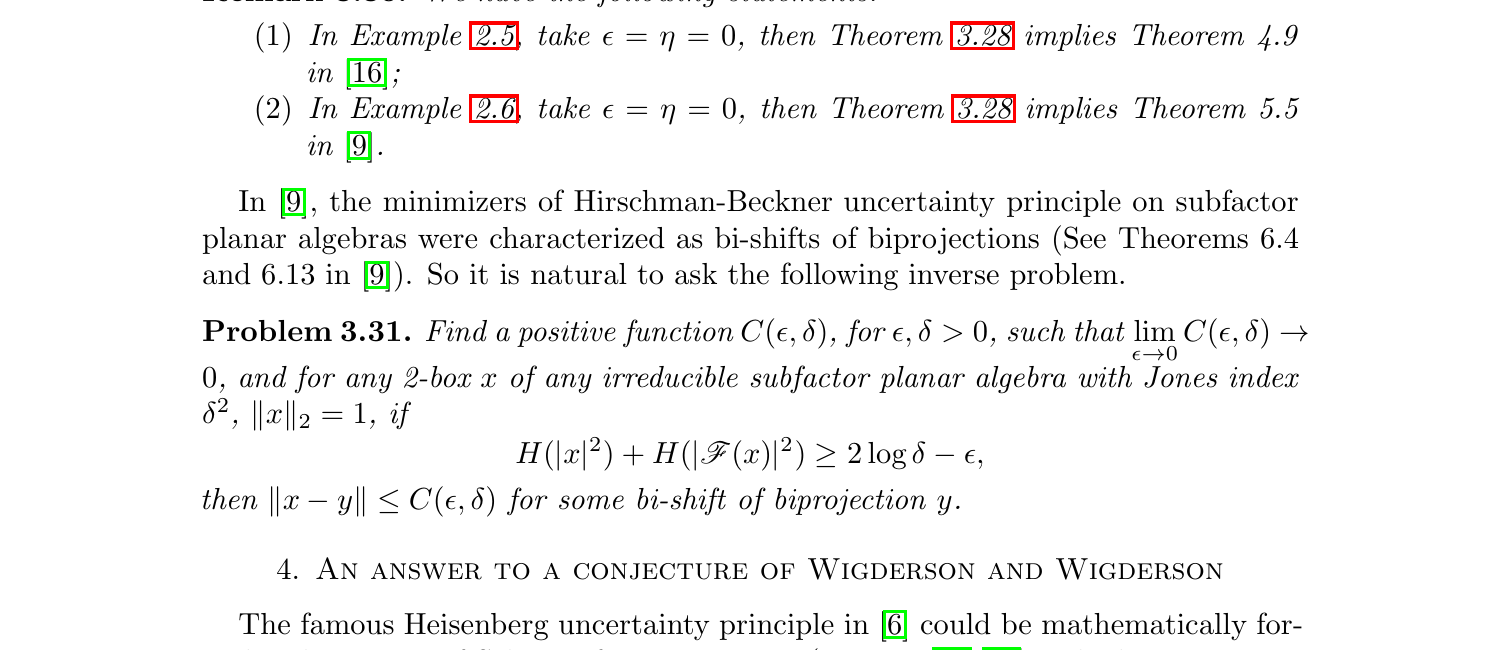
\includegraphics[width=.94\textwidth]{figures/problem331_crop.png}
\end{center}

Immediately above the problem, the source recalls that bi-shifts are exactly
the minimizers.  More decisively, its Corollary~3.29 with the smoothing
parameters set to zero gives
\begin{equation}\label{eq:uncertainty}
 H(|x|^2)+H(|\F(x)|^2)\ge 2\log\delta
 \qquad (\|x\|_2=1).
\end{equation}
Thus \eqref{eq:source} does not express near-minimality: by
\eqref{eq:uncertainty}, it holds for every normalized $x$ and every
$\epsilon>0$.

\section{Counterexample}

\begin{theorem}\label{thm:counterexample}
No function $C$ with the property required by Problem~3.31 exists.  In the
irreducible group-subfactor planar algebra associated with
$G=\mathbb Z_2$, there is a normalized $2$-box $x$ satisfying the premise for
every $\epsilon>0$ whose distance from every bi-shift of a biprojection is at
least $1/\sqrt2$ in the $2$-norm and at least $1/2$ in the operator norm.
\end{theorem}

\section{Proof intuition}

The group-subfactor example recovers ordinary finite Fourier analysis.  On
$\mathbb Z_2$, bi-shifts of subgroup indicators form only four complex
lines: the two coordinate lines and the two Fourier-character lines.  Choose
a vector whose position and Fourier probability distributions are both
uniform but whose relative phase keeps it off all four lines.  It has entropy
strictly \emph{above} the minimum, yet the printed lower-bound premise accepts
it for every error tolerance.  A function tending to zero cannot bridge its
fixed distance to the four minimizer lines.

\section{Proof}

\begin{proof}[Proof of Theorem \ref{thm:counterexample}]
Jiang, Liu, and Wu explain that finite abelian group subfactors recover the
classical Fourier uncertainty principle~\cite[Sections 2 and 8]{JLW}.  For
$G=\mathbb Z_2$, identify the relevant $2$-box with $\C^2$ in its orthonormal
delta basis.  The Jones index is $2$, so $\delta=\sqrt2$, and the normalized
Fourier transform is
\[
 \F(a,b)=\frac1{\sqrt2}(a+b,a-b).
\]
Set
\[
 x=\frac1{\sqrt2}(1,i).
\]
Then $\|x\|_2=1$, and
\[
 \F x=\frac12(1+i,1-i).
\]
Consequently, both $|x|^2$ and $|\F x|^2$ are the uniform probability vector
$(1/2,1/2)$.  With $H(p)=-\sum_jp_j\log p_j$,
\begin{equation}\label{eq:entropy}
 H(|x|^2)+H(|\F x|^2)=2\log2.
\end{equation}
Since $2\log\delta=\log2$, equation \eqref{eq:entropy} implies
\eqref{eq:source} for every $\epsilon>0$.

It remains to quantify the failure of the conclusion.  In a finite group
subfactor, every bi-shift has the form
\[
 c\sum_{h\in K}\chi(h)\,\delta_{hg},
\]
where $K\le G$, $g\in G$, $\chi$ is a one-dimensional representation of
$K$, and $c\in\C$~\cite[Proposition 8.1]{JLW}.  The only subgroups of
$\mathbb Z_2$ are $\{0\}$ and $\mathbb Z_2$.  Therefore the set of all
bi-shifts is the union of the four complex lines
\begin{equation}\label{eq:lines}
 \operatorname{span}(1,0),\quad
 \operatorname{span}(0,1),\quad
 \operatorname{span}(1,1),\quad
 \operatorname{span}(1,-1).
\end{equation}

\newpage
For a unit vector $u$ spanning any line in \eqref{eq:lines}, direct
calculation gives $|\langle x,u\rangle|=1/\sqrt2$.  Hence
\[
 \inf_{y\text{ a bi-shift}}\|x-y\|_2
 =\sqrt{1-\frac12}=\frac1{\sqrt2}.
\]
If the unadorned norm in Problem~3.31 denotes the operator norm, the same
four-line calculation in $\ell^\infty_2$ gives the lower bound $1/2$: it is
$1/\sqrt2$ for either coordinate line, while the smallest disk containing
the two target coordinates for either character line has radius $1/2$.

Now suppose the requested $C$ existed.  Since
$C(\epsilon,\sqrt2)\to0$, choose $\epsilon>0$ with
$C(\epsilon,\sqrt2)<1/2$.  The vector $x$ satisfies the premise, but no
bi-shift satisfies the required conclusion in either natural norm.  This is
a contradiction.
\end{proof}

\section{Correction and scope}

The standard stability question for a lower-bound inequality asks that the
quantity be at most the minimum plus a small error.  The likely intended
hypothesis is
\begin{equation}\label{eq:corrected}
 H(|x|^2)+H(|\F(x)|^2)\le 2\log\delta+\epsilon.
\end{equation}
The present counterexample does not address the genuinely interesting
uniform stability problem under \eqref{eq:corrected}; it refutes only
Problem~3.31 exactly as printed.

The source also asks in Problem~4.7 for a sharp Fourier-norm constant on
$\mathbb R$.  A separate deep attempt checked Gaussian tests, equality
conditions, comb limits, a R\'enyi reformulation, and the Euler--Lagrange
equation.  The Gaussian does not attain the source lower bound because the
sharp Hausdorff--Young and interpolation equality conditions are
incompatible.  No full answer to Problem~4.7 is claimed here.

\section{Verification and novelty}

The counterexample was checked in two independent ways: first, the printed
premise was compared directly with the source's Corollary~3.29; second, all
four $\mathbb Z_2$ bi-shift lines were enumerated using the finite-group
classification and their exact distances from $x$ were computed.  No
numerical approximation is used as proof.

The four lightweight run indexes had no entry for arXiv:2107.09057 or this
sign obstruction.  Bounded primary-source searches on 13 August 2026 used
the exact Problem~3.31 wording, its entropy inequality, and stability of
bi-shifts of biprojections.  They found no correction or later treatment.

\medskip
\noindent\textbf{Human-review recommendation.}
High priority but quick: verify the classical $\mathbb Z_2$ normalization and
confirm from the typeset source that the sign is indeed ``$\ge$''.  The
logical obstruction already follows from Corollary~3.29, independently of
the explicit distance calculation.

\begin{thebibliography}{9}
\bibitem{source}
J.~Wu, \emph{Quantum smooth uncertainty principles for von Neumann
bi-algebras}, arXiv:2107.09057 (2021), Problem~3.31.

\bibitem{JLW}
C.~Jiang, Z.~Liu, and J.~Wu,
\emph{Noncommutative uncertainty principles},
J. Funct. Anal. 270 (2016), 264--311; arXiv:1408.1165.
\end{thebibliography}

\end{document}
